\documentclass{llncs}
\usepackage{enumerate}
\usepackage{amssymb,amsmath}
\usepackage{enumitem}
\usepackage{verbatim}

% xelatex
%\usepackage{fontspec}
%\usepackage{xunicode}
%\usepackage{xltxtra}

%valodas. nez, vai vajag
%\usepackage{polyglossia}
%\setdefaultlanguage{english}
%\setotherlanguages{latvian,russian}


\usepackage[numbers]{natbib}

\renewcommand\bibname{\refname} %renames Bibliography -> References

%fixes underscore error in bibliography urls
\usepackage{url}
\let\harvardurl\url

% bibliography
%\usepackage{csquotes}
%\usepackage[
%    backend=biber,
%    style=numeric-comp,
%    sorting=none,
%    natbib=true,
%    url=false,
%    doi=true%,
%    %eprint=false
%]{biblatex}
%\addbibresource{bibliography.bib}

%images
\usepackage{graphicx}
\usepackage{float}

%dal�?ana kolonn�s
\usepackage{multicol}

%papildus matem�tika
\usepackage{mathtools}


\newcommand{\norm}[1]{\left\| #1 \right\|}

%iespie? tekstu ar? pie liel?m bild?m
\renewcommand\floatpagefraction{.9}
\renewcommand\topfraction{.9}
\renewcommand\bottomfraction{.9}
\renewcommand\textfraction{.1}

%\usepackage{microtype}

\usepackage[font={small,it}]{caption}


\begin{document}


\title{On the Hierarchy Classes of Finite Ultrametric Automata}


\author{
Rihards Kri\v slauks, Kaspars Balodis}
\institute{University of Latvia Faculty of Computing,\\ Rai\c na bulv\= aris 19, Riga, LV-1459, Latvia
}

\maketitle

\begin{abstract}
This paper explores the language classes that arise with respect to the head count of a finite ultrametric automaton. First we prove that in the one-way setting there is a language that can be recognized by a one-head ultrametric finite automaton and cannot be recognized by any $k$-head non-deterministic finite automaton. Then we prove that in the two-way setting the class of languages recognized by ultrametric finite $k$-head automata is a proper subclass of the class of languages recognized by $(k+1)$-head automata. Ultrametric finite automata are similar to probabilistic and quantum automata and have only just recently been introduced by Freivalds. We introduce ultrametric Turing machines and ultrametric multi-register machines to assist in proving the results.
\end{abstract}



\section{Introduction} 
Ultrametric finite automata and ultrametric Turing machines were first introduced by \citet{Freivalds2012}. This development has been followed by several papers in which various aspects of these machines are studied in depth. \citet{ KasparsBalodis2013} have studied the descriptional complexity of ultrametric automata. They showed that ultrametric automata can achieve an exponential advantage in terms of the number of states required when compared with  equivalent deterministic automata. \citet{Krislauks2013} have studied the reversal complexity of ultrametric Turing machines.

Ultrametric machines are similar to probabilistic machines, with the difference  that for ultrametric machines it is not necessary for amplitudes (which are the equivalent of probabilities in probabilistic automata) to be within the range of 0 and 1. Instead, general $p$-adic numbers are used. We should note that in \citep{Turakainen1969}, a similar generalization of probabilistic automata was introduced, where "probabilities" can be arbitrarily large numbers, and the acceptance criterion is whether the probability to be in an accepting state is greater than a given threshold. Furthermore, it was shown that this generalization is in fact equivalent to  probabilistic automata. However, unlike the concepts used for these pseudo-probabilistic machines, the definition of ultrametric machines uses the concept of a $p$-adic norm.

It can be argued that the definition introduced by Freivalds is natural, because in 1916, Alexander Ostrowski proved that any non-trivial absolute value on the rational numbers $Q$ is equivalent to either the usual real absolute value or a $p$-adic absolute value.
This result demonstrates that using $p$-adic numbers is not merely one of many possibilities to generalize the definition of deterministic algorithms, but rather the only remaining possibility not yet explored \citep{Freivalds2012}.
Additionally, useful properties have been proven for the definition of ultrametric machines---\citet{KasparsBalodis2013} proved that the language class recognized by regulated $p$-adic machines coincides with the class of regular languages.

In this paper, we address the question of the language hierarchy associated with the number of heads of ultrametric multi-head automata.
Several results can be found in the literature that  consider deterministic, nondeterministic, and probabilistic finite automata in both---two-way and one-way---cases \citep{Holzer2009, Yao1978, Monien1980, Macarie1995}. This paper examines whether similar results regarding the separation in classes with respect to the head count can be achieved for ultrametric multi-head finite automata. Other results consider the relationships of the language classes recognized by ultrametric and classical automata.

\section{$p$-adic numbers}

$p$-adic numbers are discussed in more detail in \citep{Madore}. The use of $p$-adics in other sciences can be seen in \citep{Kozyrev2006,Dragovich2009}.
Here, we only restate the definition of the $p$-adic absolute value.

For every non-zero rational number $\alpha$ there exists a unique prime factorization $\alpha = \pm 2^{\alpha_2}3^{\alpha_3}5^{\alpha_5}7^{\alpha_7} \cdots$ where $\alpha_i \in \mathbb{Z}$.
\begin{definition}
 The $p$-adic absolute value (also called the \textbf{$p$-norm}) of a rational number $\alpha = \pm 2^{\alpha_2}3^{\alpha_3}5^{\alpha_5}7^{\alpha_7} \cdots$ is 
\[
\|\alpha\|_p = \begin{cases}
p^{-\alpha_p}, &\textrm{if } \alpha \neq 0 \\
0, &\textrm{if } \alpha = 0.
\end{cases}
\]
\end{definition}

%vecaa atsauce \citep{V.S.Vladimirov1995,Kozyrev2006,Dragovich2009}.

\section{One-way multi-head automata}
\subsection{Definitions}
%Ultrametric automata are defined as in \citep{KasparsBalodis2013}.
We extend the definition of ultrametric automata given in \citep{KasparsBalodis2013} by adding rejecting states.
\begin{definition}
A finite one-way $p$-ultrametric one-head automaton  ($1\mathit{u_pfa}$ or $1\mathit{u_pfa}(1)$) is a sextuple
$\langle S, \Sigma, s_0, \delta, Q_A, Q_R \rangle$ where
\begin{itemize}
  \item $S$ is a finite set---the set of states,
  \item $\Sigma$ is a finite set ($\$ \notin \Sigma$)---input alphabet,
  \item $s_0:S \rightarrow \mathbb{Q}_p$ is the initial amplitude distribution,
  \item $\delta: \left( \Sigma \cup \left\{ \$ \right\} \right) \times S \times S \rightarrow \mathbb{Q}_p$ is the transition function,
  \item $Q_A, Q_R \subseteq S$ are the sets of accepting and rejecting states, respectively.
\end{itemize}
The automaton works as follows:
At every timestep, each of its states has an associated $p$-adic number called its amplitude.
The automaton starts with an initial amplitude distribution $s_0$.
It subsequently proceeds by processing the input word's $w = w_1 \ldots w_n$ symbols one at a time.
The amplitude distribution after processing the $i$-th symbol is denoted as $s_i$, with
$s_i(y) = \sum_{x \in S}{s_{i-1}(x) \cdot \delta \left( w_i, x, y \right) }$ for every $y \in S$.
After the $n$-th symbol,the end marker $\$$ is similarly processed, obtaining the final amplitude distribution $s_{n+1}$.
If the sum of the $p$-norms of final amplitudes over accepting states is greater than the sum of final amplitudes over rejecting states, i.e. if $\sum_{x \in Q_A}{\left\| s_{n+1}(x) \right\|_p} > \sum_{x \in Q_R}{\left\| s_{n+1}(x) \right\|_p}$, then the word $w$ is said to be accepted, otherwise---rejected.
\end{definition}

A two-way $k$-head finite automaton consists of an input tape containing the input word on which the heads of the automaton can move freely in both directions, not crossing the endmarkers. The tape is read-only. We use the standard definition for the two-way $k$-head non-deterministic finite automaton:
\begin{definition}[\citep{Holzer2009}]
A two-way non-deterministic $k$-head finite automaton ($2\mathit{nfa}(k)$) is a sextuple $\langle S, \Sigma, k, s_0, \delta, F \rangle$, where
\begin{itemize}
	\item $S$ is a finite set---the set of states,
	\item $\Sigma$ is a finite set ($ \triangleright,\triangleleft \notin \Sigma$)---the input alphabet ($\triangleright$ and $\triangleleft$ are the left and right endmarkers, respectively),
	\item $k\geq 1$ is the number of heads, 
	\item $s_0\in S$ is the starting state,
	\item $\delta: S \times \left( \Sigma \cup \left\{ \triangleright, \triangleleft \right\} \right)^k \rightarrow 2^{ S \times \left\{-1,0,1\right\}^k }$ is the partial transition function. Whenever $\left( s', (d_1, \dots, d_k) \right) \in \delta \left( s, (a_1, \dots, a_k) \right)$ is defined, then $d_i \in \{0, 1\}$ if $a_i=\triangleright$, and $d_i \in \{-1, 0\}$ if $a_i=\triangleleft$, for $1 \leq i \leq k$,
	\item $F \subseteq S$ is the set of accepting states.
\end{itemize}
\end{definition}


%At the beginning of work, a $2\mathit{nfa}(k)$ has all of its heads placed on the left endmarker. A configuration of a $2\mathit{nfa}(k)$ in some moment in time $t\geq 0$ is a 3-tuple $c_t=\left(w,s,p\right)$ where $w$ is the input word, $s\in S$ is the current state and
%$p = \left( p_1, \ldots, p_k \right) \in \left\{ 0, \ldots, |w| +1 \right\}^k $
%gives the current head positions.
%The initial configuration for input $w$ is set to $\left(w,s_0,\left(0,\ldots,0\right)\right)$.
%The automaton ends its work when the transition function $\delta$ is not defined for the current configuration. A transition from one configuration to the next is denoted by $\vdash$. A transition
%$\left( w, s, \left( p_1, \ldots, p_k \right) \right) \vdash \left( w, s', \left( p_1+d_1, \ldots, p_k+d_k \right) \right)$
%is valid iff
%$\left( s', \left(d_1, \ldots, d_k \right) \right) \in \delta \left( s, \left( a_{p_1}, \ldots a_{p_k} \right) \right)$
%where $w = a_1a_2 \ldots a_n$ is the input word and $a_0=\triangleright$ and $a_{n+1}=\triangleleft$. The reflexive transitive closure of $\vdash$
%is denoted by $\vdash^*$.
%
%A $2\mathit{nfa}(k)$ accepts a word $w$ iff there exists a sequence of configurations that results in automaton stopping in an accepting state if the input tape contains
%$\triangleright w \triangleleft$. The language $L(M)$ accepted by $M$ consists of those and only those words that are accepted by $M$.  More precisely,   
%\begin{multline*}
%	L(M)=\left\{ w \in \Sigma^* | \left(w,s_0,\left(0,\dots,0\right)\right) \vdash^* \left(w,s,\left(p_1,\dots,p_k\right)\right), s \in F,\right.\\
%	\left.\textrm{and } M \textrm{ halts in } \left(w,s,\left(p_1,\ldots,p_k\right)\right)\right\}.
%\end{multline*}


If for any state and $k$-tuple of symbols the transition function $\delta$ is either undefined or singleton, 
then the automaton is said to be deterministic ($2\mathit{dfa}(k)$).
If the heads of the automaton never move left, then the automaton is defined to be one-way. Nondeterministic and deterministic one-way $k$-head automata are denoted by $1\mathit{nfa}(k)$ and $1\mathit{dfa}(k)$, respectively.

\subsection{Relation to classical automata}
Strict hierarchies of classes have been shown for both one-way multi-head deterministic and nondeterministic automata with regard to the head count of the automata \citep{Holzer2009,Yao1978}.
In 1978, \citet{Yao1978} used the language
\[
	L'_k = \left\{w_1\$w_2\$ \ldots \$w_{2k} \middle| w_i \in \left\{a,b\right\}^* \wedge w_i = w_{2k+1-i} \textrm{ for all } 1 \leq i \leq k \right\}
\]
to prove the separation of the class of languages that can be recognized by a $1\mathit{dfa}(k)$ from the class that can be recognized by a $1\mathit{dfa}(k+1)$.

We will consider a similar language,   $L_k$.
\begin{theorem}
For every $k \geq 1 \in \mathbb{N}$, there exists a language $L_k$ such that:
\begin{enumerate}[label={(\arabic*)}]
	\item for every prime $p$ there exists a $1\mathit{u_pfa}(1)$ that recognizes $L_k$,
	\item $L_k$ cannot be recognized by any $1\mathit{nfa}(k)$.
\end{enumerate}
\end{theorem}
\begin{proof} Let $n={k\choose 2}+1$. The sought language is
\[
L_k = \left\{ w_1 1 w_2 1 \ldots 1 w_{2n} \middle|
		w_i \in \left\{ 0^m | m \geq 1 \right\} \wedge
		w_i = w_{2n-i+1} 
		 \right\}.
\]
We will now prove that $L_k$ satisfies the points of our theorem.

$(1)$ We show that for an arbitrary language $L_k$, a $1\mathit{u_pfa}(1)$ can be built for every prime number $p$. The automaton starts in $n$ different starting states $q_{1,1,1},q_{1,2,1},\ldots,q_{1,n,1}$ with amplitude $1$. Each of these states begins a computational path that is intended to accumulate amplitude in one of $n$ different rejecting states $q_{2n,1,2},q_{2n,2,2},\ldots,q_{2n,n,2}$. Every branch contains two kinds of states---states of the 1st group $q_{i,j,1}$ are responsible for generating amplitudes,  and states of the 2nd group $q_{i,j,2}$ are intended for amplitude accumulation, $i \in \left[1, 2n \right], j \in \left[1, n \right]$.

If $0$ is read from the input and the automaton is in one of the 1st group states $q_{i,j,1}$, where $i \leq n$, then the amplitude of the state remains the same and with amplitude $1$ the automaton goes to a 2nd group state, $q_{i,j,2}$. By doing so, the state's accumulated amplitude is added to $q_{i,j,2}$. If $0$ is read in a 2nd  group state $q_{i,j,2}$, the state's amplitude remains the same. If $1$ is read in a 1st group state $q_{i,j,1}$, where $i < n$, then the automaton with amplitude $j + 1$ transitions to $q_{i + 1,j,1}$, thereby transitioning there with amplitude $(j + 1) \cdot \left| q_{i + 1,j,1} \right|$ (by $|q_i|$, we denote the amplitude of the state $q_i$).
In contrast, if $0$ is read in the 1st group state $q_{i,j,1}$, where $i > n$, the amplitude of the state remains unchanged and the transition to $q_{i,j,2}$ is made with amplitude $-1$. If $1$ is read in the 1st group state $q_{i,j,1}$, where $i \geq n$, the transition to $q_{i + 1,j,1}$ is made with amplitude $-(j + 1)$. If $1$ is read in a 2nd group state, a transition is made from $q_{i,j,1}$ to $q_{i + 1,j,1}$, with amplitude $1$. The exception is the last column of states,   $q_{2n,j,1}$ and $q_{2n,j,2}$, which are responsible for reading in the last block of the word. In this case, the transition if $1$ is read is not defined. A schematic representation of the described automaton is presented  in Fig. \ref{fig:1pfa}.

As a result, if a word $0^{a_1}10^{a_2}10^{a_3}1\ldots 10^{a_{2n}}$ was read, then each of the rejecting states $q_{2n,j,2}$ has accumulated an amplitude equal to
\[
	a_1 + a_2 \cdot (j + 1) + a_3 \cdot (j + 1)^2 + \cdots + a_n \cdot (j + 1)^{n - 1} - a_{n+1} \cdot (j + 1)^{n - 1} - a_{n+2} \cdot (j + 1)^{n - 2} - \cdots - a_{2n},
\]
which is equal to $0$ if the word belongs to the language; i.e. if
\[
	a_1 = a_{2n} \wedge a_2 = a_{2n-1} \wedge \ldots \wedge a_n = a_{n+1}.
\]
It follows that a word is in $L_k$ iff the following equations hold:
\begin{gather*}
\allowdisplaybreaks
	\begin{cases}
		a_1 + a_2 \cdot 2 + a_3 \cdot 2^2 + \cdots + a_n \cdot 2^{n - 1} - a_{n+1} \cdot 2^{n - 1} - a_{n+2} \cdot 2^{n - 2} - \cdots - a_{2n} = 0 \\
		a_1 + a_2 \cdot 3 + a_3 \cdot 3^2 + \cdots + a_n \cdot 3^{n - 1} - a_{n+1} \cdot 3^{n - 1} - a_{n+2} \cdot 3^{n - 2} - \cdots - a_{2n} = 0\\
		% a_1 + a_2 \cdot 4 + a_3 \cdot 4^2 + \cdots + a_n \cdot 4^{n - 1} - a_{n+1} \cdot 4^{n - 1} - a_{n+2} \cdot 4^{n - 2} - \cdots - a_{2n} = 0\\
		\cdots \\
		\begin{split}
		a_1 + a_2 \cdot (n + 1) + a_3 \cdot (n + 1)^2 + \cdots + a_n \cdot (n + 1)^{n - 1} - a_{n+1} \cdot (n + 1)^{n - 1} \\
		\qquad- a_{n+2} \cdot (n + 1)^{n - 2} - \cdots - a_{2n} = 0\\
		\end{split}
	\end{cases}\\
\intertext{rewriting}
	\begin{cases}
		(a_1 - a_{2n}) + 2 \cdot (a_2 - a_{2n-1}) + 2^2 \cdot (a_3 - a_{2n-2}) + \cdots + 2^{n - 1} \cdot (a_n - a_{n+1}) = 0\\
		(a_1 - a_{2n}) + 3 \cdot (a_2 - a_{2n-1}) + 3^2 \cdot (a_3 - a_{2n-2}) + \cdots + 3^{n - 1} \cdot (a_n - a_{n+1}) = 0\\
		% (a_1 - a_{2n}) + 4 \cdot (a_2 - a_{2n-1}) + 4^2 \cdot (a_3 - a_{2n-2}) + \cdots + 4^{n - 1} \cdot (a_n - a_{n+1}) = 0\\
		\cdots \\
		\begin{split}
		(a_1 - a_{2n}) + (n + 1) \cdot (a_2 - a_{2n-1}) + (n + 1)^2 \cdot (a_3 - a_{2n-2}) + \cdots \\
		\qquad+ (n + 1)^{n - 1} \cdot (a_n - a_{n+1}) = 0\\
		\end{split}	
	\end{cases}
\end{gather*}

We see that the coefficients of the system form a Vandermonde matrix. Therefore, its determinant is non-zero, and since the given system is homogeneous, only the trivial solution exists.

However, if the word does not belong to $L_k$, then no more  than $4$ lines can hold true. However, even in this case at least one line will exist that is not equal to $0$.
Otherwise the system would have a nontrivial solution.
Therefore, a word belongs to $L_k$ iff the sum of the final amplitude norms of the rejecting states is greater than $0$.

By adding an accepting state with a sufficiently small norm of the amplitude (decreasing as the length of the word increases) it is possible to make the automaton accept the language $L_k$.

$(2)$ Proven by \citet{Freivalds1979}, a proof for a similar language can also be found in \citep{Yao1978}. The idea of this proof relies on the fact that any two heads that have been used to compare a pair cannot be used to compare another pair. This implies that if the number of block pairs in a word $n$ is greater than the number of pairs of heads ${k\choose 2}$, then the language cannot be recognized with $k$ heads.
\qed
\end{proof}

\begin{figure}
\centering
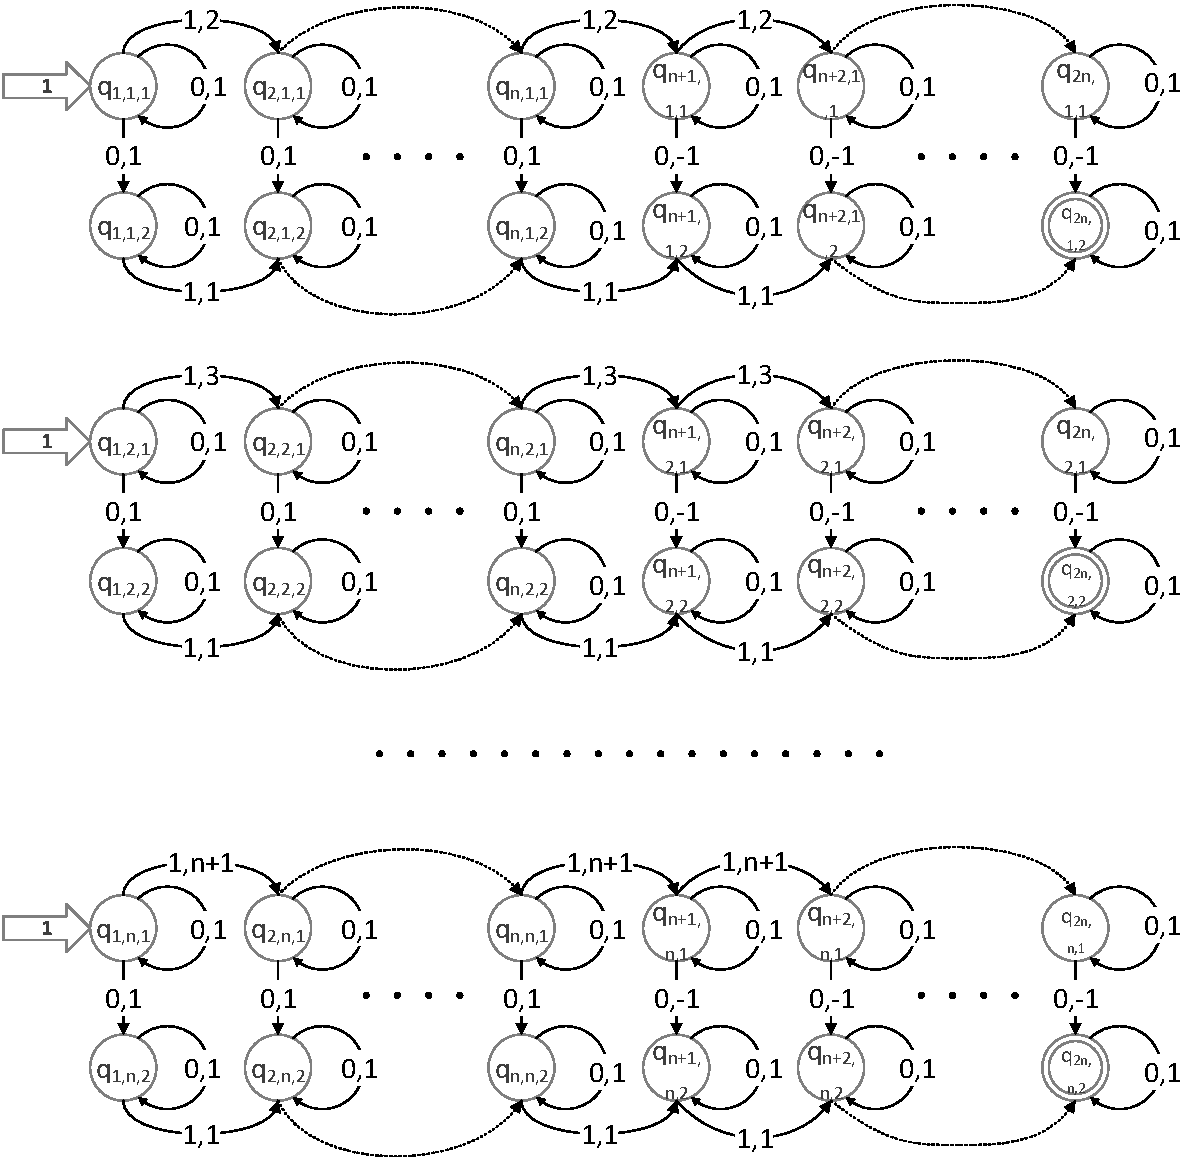
\includegraphics[width=\textwidth]{Img/1pfa.pdf}
\caption{Automaton for recognizing $0^n10^m10^h1 \cdots 10^h10^m10^n$. Double-circled states are rejecting. Large arrows with labels in them show the amplitude distribution when the automaton starts. Small labelled arrows show transitions. A label $(a, b)$ indicates that if the automaton reads $a$, transition with amplitude $b$ should be made.}
\label{fig:1pfa}
\end{figure}

%  n�kamais lieki t�r� vietu?
% It should be noted that to recognize $L_k$, a constant number of heads is sufficient for a probabilistic automaton as well. \citet{Freivalds1982} has proven that for every $\epsilon > 0$ there exists a $1pfa$ that accepts every word in $L_k$ with probability $1$ and rejects others with probability $1 - \epsilon$.

% \section{One-way multi-head automata}
% neb�s

\section{Two-way automata}
\subsection{Definitions}
Ultrametric multi-head automata are defined by generalizing the definition of ultrametric one-head one-way automata in a natural way. The definition of multi-head automata due to \citet{Holzer2009} is used as well.

\begin{definition}
A finite $k$-head two-way $p$-ultrametric automaton ($2\mathit{u_pfa}(k)$) is a septuple $\langle S, \Sigma, k, s_0, \delta, Q_A, Q_R \rangle$ where
\begin{itemize}
	\item $S$ is a finite set of states,
	\item $\Sigma$ is a finite set ($ \triangleright,\triangleleft \notin \Sigma$)---the input alphabet ($\triangleright$ and $\triangleleft$ are the left and right endmarkers, respectively),
	\item $k\geq 1$ is the number of heads, 
	\item $s_0:S \rightarrow \mathbb{Q}_p$ is the initial distribution of amplitudes,
	\item $\delta: S \times \left( \Sigma \cup \left\{ \triangleright, \triangleleft \right\} \right)^k \times S \times \left\{-1,0,1\right\}^k \rightarrow \mathbb{Q}_p$ is the partial transition function.  Whenever $\delta \left( s, (a_1, \dots, a_k), s', \left( d_1, \dots, d_k \right) \right)$ is defined and not equal to $0$, then $d_i \in \{0, 1\}$ if $a_i=\triangleright$, and $d_i \in \{-1, 0\}$ if $a_i=\triangleleft$, for $1 \leq i \leq k$,
	\item $Q_A, Q_R \subseteq S$ are the sets of accepting and rejecting states, respectively.
\end{itemize}
\end{definition}

$2\mathit{u_pfa}(k)$ works in a similar way as $1\mathit{u_pfa}$, with the exception that the automaton now has $k$ heads that can move freely, as in  a $2\mathit{nfa}(k)$. In contrast to  $1\mathit{u_pfa}$, amplitudes are now given for a pair consisting of the positions of the heads and a state. The amplitude of the state $y \in S$ with heads in positions
$\left( p_1, \ldots, p_k \right) \in \left\{ 0, \ldots, |w| +1 \right\}^k $ on the word $w = a_1 \dots a_n$
after the $i$-th operation is given by
\[
s_i (y, (p_1, \ldots, p_k)) =
\sum_{\mathclap{\substack{ x \in S, 
		p'_1, \ldots, p'_k \in \left\{ 0, 1, \dots, n+1 \right\}: \\
		\delta \left( x, \left(a_{p'_1}, \dots, a_{p'_k}\right), y, \left(p_1 - p'_1, \dots, p_k - p'_k \right) \right) \text{ is defined}
		}}}
	{
	s_{i-1}\left(x, \left(p'_1, \ldots, p'_k\right)\right)
	\cdot
	\delta \left( x, \left(a_{p'_1}, \dots, a_{p'_k}\right), y, \left(p_1 - p'_1, \dots, p_k - p'_k \right) \right) }
\]

\vspace{-2mm}
Similarly as before, the acceptance of a word is determined by comparing the final amplitude $p$-norm sum of the accepting and rejecting states. That is, the word is accepted iff
\[
\sum_{x \in Q_A}{ \left\| \mkern42mu \sum_{\mathclap{\substack{ 
		i \in \mathbb{N}, \\
		(p_1, \ldots, p_k) \in F_i (x) }}}
	{ s_{i}(x, (p_1, \ldots, p_k))} \right\|_p } >
\sum_{x \in Q_R}{ \left\| \mkern42mu \sum_{\mathclap{\substack{ 
		i \in \mathbb{N}, \\
		(p_1, \ldots, p_k) \in F_i (x) }}}
	{ s_{i}(x, (p_1, \ldots, p_k))} \right\|_p }
\]
%\[
%\sum_{x \in Q_A}{ \left\| \mkern150mu \sum_{\mathclap{\substack{ 
%		(p_1, \ldots, p_k) \in \left\{ 0, 1, \dots, n+1 \right\}, 
%		i \in \mathbb{N} : \\
%		\textrm{ the automaton halts in the } i \textrm{-th step in the state } x \\
%		\textrm{ with the heads in positions } (p_1, \ldots, p_k) }}}
%	{ s_{i}(x, (p_1, \ldots, p_k))} \mkern13mu \right\|_p } >
%\sum_{x \in Q_R}{ \left\| \mkern150mu \sum_{\mathclap{\substack{ 
%		(p_1, \ldots, p_k) \in \left\{ 0, 1, \dots, n+1 \right\}, 
%		i \in \mathbb{N} : \\
%		\textrm{ the automaton halts in the } i \textrm{-th step in the state } x \\
%		\textrm{ with the heads in positions } (p_1, \ldots, p_k) }}}
%	{ s_{i}(x, (p_1, \ldots, p_k))} \mkern13mu \right\|_p }
%\]
where $(p_1, \dots, p_k) \in F_i(x)$ iff the automaton with some amplitude halts in the $i$-th step in the state $x$ with the heads in positions $p_1, \dots, p_k$.
We require the automaton to be built in such a way that these norms of the (possibly infinite) sums converge for every $w \in \Sigma^*$.

The class of languages recognized by $2\mathit{u_pfa}(k)$ is denoted $2\mathit{U_pFA}(k)$.

Ultrametric Turing machines are defined to be used as a device to assist in proving results regarding multi-head automata classes. We modify the definition for Turing machine by \citet{Hopcroft1979}.
\begin{definition}
A $p$-ultrametric Turing machine with $k$ work tapes ($u_ptm(k)$ or simply $u_ptm$) is an octuple $M= \langle Q, \Sigma, b, \Gamma, q_0, \delta, Q_A, Q_R \rangle$ where:
\begin{itemize}
	\item $Q$ is a nonempty set of states,
	\item $\Sigma$ is a nonempty set---the input alphabet,
	\item $b \notin \Sigma$  is the ``empty'' symbol,
	\item $\Gamma \supseteq \Sigma\cup\{b\}$ is the working alphabet,
	\item $q_0 : Q \rightarrow \mathbb{Q}_p$ is the initial amplitude distribution,
	\item $\delta: Q \times \Gamma^k \times Q \times \left( \Gamma \times \{-1,0,1\} \right)^k \rightarrow \mathbb{Q}_p $ is a partially-defined transition function where $-1$ denotes moving the head to the left, $1$  denotes moving the head  to the right, $0$   denotes not moving the head, and $\mathbb{Q}_p$ is the amplitude of the transition,
	\item $Q_A, Q_R \subseteq S$ are the sets of accepting and rejecting states, respectively.
\end{itemize}
\end{definition}

The class of languages recognized by a $u_ptm$ is denoted $U_pTM$.

Similarly, as with ultrametric multi-head automata, the  machine with a given amplitude is in one of its possible configurations. However, now the configuration consists of the state of the finite control, the position of the $k$ heads,  and the contents of all $k$ tapes. The amplitude with which the machine is in one of its configurations in the $i$-th step is computed analogously as in the case with ultrametric multi-head automata. The criteria for acceptance are analogous to those of ultrametric multi-head automata.
%(j�iev�ro tikai, ka tagad autom�ta konfigur�cij� ietilpst ar� no lentes saturs, un amplit�da tiek piek�rtota tam kombin�cij� ar vad�bas bloka st�vokli).

Ultrametric multi-register automata are also used as an intermediate device for proofs.
\begin{definition}
A finite $p$-ultrametric $k$ register automaton (also referred to as a machine) ($2u_pra(k)$) consists of a $p$-ultrametric finite control and $k$ registers that can hold natural numbers. The automaton begins with the input number in the first register with the specified starting amplitude distribution in some of its states . A predicate $\stackrel{?}{=} 0$ and the operations $+1$ or $-1$ can be applied to a register. Each of the transitions of the finite control can have a predicate or an operation associated with it that is triggered when the transition is made. Acceptance criteria are analogous to those of ultrametric automata.
\end{definition}



\subsection{Simulation of ultrametric automata by ultrametric Turing machines}

In this subsection, we will show how to simulate an ultrametric multi-head automaton by an ultrametric Turing machine.
The techniques used here are similar to the techniques used by \citet{Macarie1995} for probabilistic automata.

Without loss of generality, we can assume that the simulated automaton has at most $2$ transitions from each state and input symbol.
We will show how to construct a $p$-ultrametric $2$-tape Turing machine that, having received  the description of a $k$-head $p$-ultrametric automaton as an input, will accept exactly the same words as the automaton.
We will consider only automata recognizing unary languages, and we will show how to encode the description of the automaton as a word in the form $1^{2^n}, n \in \mathbb{N}$.
Furthermore, we will require that the amplitudes of the simulated automaton are $p$-constructible sets.


\begin{definition}
A set $S$ of $p$-adic numbers is $p$-constructible if there exists a $p$-ultrametric Turing machine that, having received a description of a number $x \in S$ as an input, reaches a marked state $q_u$ with amplitude $x$.
\end{definition}
%TODO aprakstam neb�tu j�b�t ar kk�du ierobe�otu garumu? cit�di ?�iet, ka nav j�gas no log-space sare���t�bas

% Teor�ma par racion�liem skait�iem neb�s
%\begin{theorem}
%The set of rational numbers is $log$-space $p$-constructible.
%\end{theorem}
%\begin{proof}
%The description of a rational number $a$ is given as
%\[
%	\triangleright a_n a_{n-1} \cdots a_1 \cdot a_0 | a_{-1} a_{-2} \cdots a_{-m} \triangleleft,
%\]
%where $|$ is a delimiting symbol, $a_i \in \{0, 1\}$ and 
%\[ %
%	a = \sum\limits_{i=-m}^n a_i \cdot 2^i
%\]
%The machine 
%\qed
%\end{proof}

A $2\mathit{u_pfa}(k)$ can be described with a binary sequence denoting, in turn: the number of states, the number of heads, the transitions between the states, and their respective amplitudes.

The simulation is performed as follows:
The $2\mathit{u_pfa}(k)$ $\mathcal{A}$ with transitions from a $p$-constructible set is simulated by a $u_ptm(2)$ $\mathcal{T}$.
$\mathcal{T}$ receives the description of $\mathcal{A}$ in unary alphabet as a word in the form $1^{2^n}, n \in \mathbb{N}$.
$\mathcal{T}$ starts by reading the input word and deterministically (making transitions with amplitude $1$) writes $n$ in binary on the second tape, where $n$ is the description of the automaton $\mathcal{A}$.
Additionally, a space of size $O(k \cdot n)$ is reserved (assuming that the length of the input word on which the automaton must be simulated does not exceed $2^n$) for $k$ counters denoting the positions of the heads of the automaton $\mathcal{A}$.
From this point forward, only the second tape will be used (we will refer to it as the work tape).

While processing the input word, the automaton $\mathcal{A}$ can be in different configurations in parallel with different amplitudes.
If $\mathcal{A}$ is in a configuration with an amplitude $a$, $\mathcal{T}$ will simulate it by being in a configuration in which the content of the work tape corresponds to the respective configuration of $\mathcal{A}$ with  the same amplitude $a$.

To show that $\mathcal{T}$ can simulate $\mathcal{A}$ in such a way, we must show that every transition of $\mathcal{A}$ can be realized by $\mathcal{T}$.
If $\mathcal{A}$ has a transition from $q_1$ to $q_2$ with an amplitude $a_1$, and from $q_1$ to $q_3$ with an amplitude $a_2$, then $\mathcal{T}$ being in a configuration corresponding to $q_1$ can make transitions to configurations corresponding to $q_2$ and $q_3$ with amplitudes $a_1$ and $a_2$, respectively.
This simulation is accomplished by $\mathcal{T}$ branching into two branches, and in both of them writing on a special place on the tape  $d_1$ or $d_2$, respectively, with an amplitude $1$, where $d_1$ and $d_2$ are the descriptions of the transitions and the amplitudes $a_1$ and $a_2$, respectively.
This is done deterministically with amplitude $1$.
Next, a subroutine is called that transitions to a marked state $q_u$ with an amplitude $a_1$ or $a_2$. (Because all transitions of $\mathcal{A}$ are $p$-constructible, there exists such a subroutine.)
Subsequently, $\mathcal{T}$ changes the work tape so that it corresponds to the respective transition (again, this is done deterministically with amplitude $1$).
Because the only transition that is accomplished with an amplitude other than $1$ is the transition to the state $q_u$, after this procedure $\mathcal{T}$ is in a configuration corresponding to $q_2$ with amplitude $a_1$, and in a configuration $q_3$ with amplitude $a_2$.





\subsection{Multi-head automata}
\citet{Monien1980} has proven that for finite deterministic and nondeterministic automata, the language class that can be recognized using $k$ heads is a proper subclass to the class of languages that can be recognized if $k+1$ heads are allowed. Using similar methods, \citet{Macarie1995} has proven the same for finite probabilistic automata. We prove here that the same holds for finite ultrametric automata.

\begin{definition}
By $\widehat{C}$, we denote the subset of a language class $C$ containing only the words in the form $1^{2^n}, n \in \mathbb{N}$, more precisely  
$\widehat{C} = \left\{ L \in C | \forall x \in L \; \exists n \in \mathbb{N} : x = 1^{2^n} \right\}$
% $\widehat{C} = \left\{ h | h \in C \wedge \exists n \in \mathbb{N} : h = 1^{2^n} \right\}$\\
\end{definition}
\begin{theorem} \label{atdalisana}
For every natural number $k$ and prime $p$:
\[
	\widehat{2\mathit{U_pFA}(k)} \subsetneqq \widehat{U_pTM}.
\]
\end{theorem}
\begin{proof}
We will construct a special $p$-ultrametric Turing machine with 2 tapes and $log$-space space complexity called $\mathcal{T}$. We will show that its recognized language cannot be recognized by a $p$-ultrametric automata with $k$ heads for any $k$.

Similarly as in the previous section,
we will construct $\mathcal{T}$ so that it simulates a $2\mathit{u_pfa}(k)$ given in its input called $\mathcal{A}$. Contrary to the previous description, the description of $\mathcal{A}$ does not directly include the input for $\mathcal{A}$. We will run $\mathcal{A}$ on the input string, i.e. on its "definition", instead.

More precisely,   $\mathcal{T}$ 1st tape contains $1^m, m \in \mathbb{N}$, $\mathcal{T}$ checks whether the word is in the form $1^{2^n}, n \in \mathbb{N}$ (if not, the word is rejected), and by taking up to $O(log(n))$ space, writes $n$'s binary representation on the 2nd tape (we will refer to it as the work tape ). It  then checks whether $n$'s binary representation is syntactically a valid $2\mathit{u_pfa}(k)$; if not, the word is rejected. Then, $\mathcal{T}$ designates a space on the work tape to be used for $k$ counters that will be used to represent $\mathcal{A}$'s head positions. Since the counter values can be in $\left\{0, \ldots, 2^n+1 \right \}$, $O(k \cdot log(2^n)) \sim O(k \cdot n)$ space is required.
All previous actions are performed deterministically. Next, $\mathcal{T}$ is run on the input string similarly as it is shown in the previous section. (The head of the first tape is not used anymore; instead, a check is performed to determine whether or not the counters corresponding to head positions are inside word boundaries.)
Consequently, $\mathcal{T}$ is with respective amplitudes in all of the possible configurations of $\mathcal{A}$ after processing the word. Afterwards, $\mathcal{T}$ checks whether the contents of the work tape suggest that $\mathcal{A}$ is in an accepting state, and halts in a rejecting state if $\mathcal{A}$ would have accepted the word; $\mathcal{T}$ halts in an accepting state if $\mathcal{A}$ would have rejected the word. Therefore, $\mathcal{T}$ yields the opposite result to that of $\mathcal{A}$ with the same amplitudes.

Let us consider the language $L(\mathcal{T})$ recognized by $\mathcal{T}$. We can see that for every $2\mathit{u_pfa}(k)$ denoted by $\mathcal{J}$, there exists a word $w$ such that it is either in $L(\mathcal{T})$ but not in $L(\mathcal{J})$, or it is in $L(\mathcal{J})$ but not in $L(\mathcal{T})$; namely,   $\mathcal{J}$'s specification. \qed
\end{proof}

Similarly, as in \citep{Macarie1995} and \citep{Monien1980}, in the following proofs we will use the function
$
	f_k : \left\{ 1^{2^n} | n \in \mathbb{N} \right\} \rightarrow \left\{ 1^{2^n} | n \in \mathbb{N} \right\} \textrm{, where } f_k( 1^{2^n}) = 1^{2^{k \cdot n}}
$.

When $f_k$ is applied to a language, we refer to the following function: $f_k(L) = \left\{ f_k(x) \middle| x\in L \right\}$.


\begin{lemma} \label{skaititaji}
For every language $L \in \widehat{U_pTM}$ that is recognized by a 2-tape $u_ptm$ in logarithmic space, there exists a natural number $u$ such that:
$
	f_u(L) \in \widehat{2\mathit{U_pFA}(3)}.
$
\end{lemma}
\begin{proof}
We will show how a $u_ptm$ denoted by $\mathcal{T}$ that recognizes $L$ can be transformed into a $u_ptm$ called $\mathcal{T'}$, which can then be replaced by a $p$-ultrametric $3$ register machine. From this, it easily follows that there exists a $2\mathit{u_pfa}(3)$ that recognizes a ``stretched"  variant of $L$, where stretching is done by $f_u$.

We will construct $\mathcal{T'}$ so that it simulates $\mathcal{T}$. $\mathcal{T'}$ will hold the following information on its work tape:
\begin{itemize}
	\item the binary information of the input word,
	\item $\mathcal{T}$ head position on the 1st tape (we will call it the input tape),
	\item $\mathcal{T}$ 2nd tape contents (we will call it the work tape) (requires $O(log n)$ space),
	\item $\mathcal{T}$ head position on the work tape.
\end{itemize}
The simulation of $\mathcal{T}$ on $\mathcal{T'}$'s work tape is less complicated than in the case of ultrametric automata, since $\mathcal{T'}$ can use the original finite control of $\mathcal{T}$, and the transitions are not required to be simulated on the tape. To simulate $\mathcal{T}$, $\mathcal{T'}$ uses only the work tape.

We can see that given $\mathcal{T'}$, a corresponding $p$-ultrametric $3$ register machine can be constructed. If the input is of the form $1^{2^n}$, then the register machine starts with $n$ in the first register and with $0$ in the remaining registers. The contents of the work tape of $\mathcal{T'}$ can be simulated by manipulating the registers of the first two stored sub-words, $v$ and $h^{rev}$, and by using  the third as an auxiliary register. To do this, we use operations ``add $1$"  and ``divide by 2", which can be carried out by using the auxiliary register.


Since a position of a multi-head automaton directly corresponds to a number in a register, and the simulated Turing machine has $log$-space space complexity, a $3$ register machine can be replaced with a $p$-ultrametric $3$ head automaton. However, since its heads cannot cross word boundaries and therefore cannot simulate arbitrarily large numbers, the input words must be sufficiently long. This is achieved by selecting a large enough $u$. \qed
\end{proof}










\begin{lemma} \label{reizinajums}
For all languages $L \in \widehat{U_pTM}$ and all $u, v \geq 1, u, v \in \mathbb{N}$:
$
	f_u(L) \in \widehat{2\mathit{U_pFA}(v)} \Rightarrow L \in \widehat{2\mathit{U_pFA}(u \cdot v)}.
$
\end{lemma}
\begin{proof}
Let the $2\mathit{u_pfa}(v)$ in the premise be $\mathcal{A}$ and the $2\mathit{u_pfa}(u \cdot v)$ in the conclusion---$\mathcal{A'}$.

Consider the operation of $\mathcal{A}$ on a word $f_u(l), l = 1^{2^n} \in L, n \in \mathbb{N}$.
The position of each of $v$ heads of $\mathcal{A}$ can be described with an integer $h_i \in \left[0, 2^{u \cdot n} -1 \right]$.
$h_i$ can be written in base $2^n$ with $u$ digits.
As the position of each head of $\mathcal{A'}$ can be described with a digit in base $2^n$, each head of $\mathcal{A}$ can be simulated with $u$ heads of $\mathcal{A'}$.
As each movement of a head of $\mathcal{A}$ corresponds to movement of heads of $\mathcal{A'}$, the respective transitions can be accomplished with equal amplitudes, and the accepting amplitudes of the words remain the same.

Note that this simulation is performed  analogously as for deterministic automata in \citep{Monien1980} and for probabilistic automata in \citep{Macarie1995}.
\qed
\end{proof}

\begin{lemma} \label{plus1}
For every language $L \in \widehat{U_pTM}$ and every $u > v > 1, u, v \in \mathbb{N}$:
\[
	f_{u+1}(L) \in \widehat{2\mathit{U_pFA}(v)} \Rightarrow f_u(L) \in \widehat{2\mathit{U_pFA}(v + 1)}.
\]
\end{lemma}
\begin{proof}
Let the $2\mathit{u_pfa}(v)$ in the premise be $\mathcal{A}$ and the $2\mathit{u_pfa}(v + 1)$ in the conclusion---$\mathcal{A'}$.

Consider the operation of $\mathcal{A}$ on a word $f_{u+1}(l), l = 1^{2^n} \in L, n \in \mathbb{N}$.

The position of each of $v$ heads of $\mathcal{A}$ on the input word can be described with an integer $h_i \in \left[0, 2^{(u + 1) \cdot n} + 1 \right]$.

We will simulate the position $h_i$ in the automaton $\mathcal{A'}$ with a head $g_i$ and an additional number $x_i \in \left[ 0, 2^n \right]$, so that $h_i = g_i + x_i \cdot 2^{u \cdot n}$.
It is evident that the values in the necessary interval can be denoted this way:
%\begin{align*}
\[
	2^{u \cdot n} + (2^n - 1) \cdot 2^{u \cdot n} =
	2^{u \cdot n} \cdot (1 + (2^n - 1)) =
	2^{u \cdot n + n} =
	2^{(u + 1) \cdot n}.
\]
%\end{align*}
All $v$ numbers $x_i$ are coded with the $(v+1)$-th head of $\mathcal{A'}$, similarly to \citep{Monien1980}. %TODO siikaak aprakstiit
This can be accomplished if sufficient space exists  on the tape of $\mathcal{A'}$, specifically if $(2^n)^v < 2^{u \cdot n}$, which holds as $v < u$.

Again, as each movement of a head of $\mathcal{A}$ corresponds to the movement of heads of $\mathcal{A'}$, the respective transitions can be accomplished with equal amplitudes, and the accepting amplitudes of the words remain the same.
% Note that this simulation again is performed analogously as for deterministic automata in \citep{Monien1980} and for probabilistic automata in \citep{Macarie1995}.
%TODO atkaartojas teksts no ieprieksheejaas lemmas, varbuut paarrakstiit // iznjemsim
\qed
\end{proof}

The result concerning the superiority of  a $k+1$ head over $k$ heads follows from the previous lemmas and Theorem \ref{atdalisana}.

\begin{theorem}
For all $k \geq 2 \in \mathbb{N}$:
\[
	\widehat{2\mathit{U_pFA}(k)} \subsetneqq \widehat{2\mathit{U_pFA}(k + 1)}.
\]
\end{theorem}
\begin{proof}
We prove from the contrary by showing that if there exists such $h \geq 2$ that $\widehat{2\mathit{U_pFA}(h)} = \widehat{2\mathit{U_pFA}(h + 1)}$, it implies $\widehat{2\mathit{U_pFA}(h \cdot (h + 1))} = \widehat{U_pTM}$, which contradicts \ref{atdalisana}.

Take $L \in \widehat{U_pTM}$ for some prime $p$. Lemma \ref{skaititaji} implies that there exists $m \in \mathbb{N}$ such that $f_m(L) \in \widehat{2\mathit{U_pFA}(3)}$. Consequently, $f_m(L) \in \widehat{2\mathit{U_pFA}(h)}$. Lemma \ref{plus1} implies that if $m > h + 1$, then $f_{m-1}(L) \in \widehat{2\mathit{U_pFA}(h + 1)} = \widehat{2\mathit{U_pFA}(h)}$.
% Take $m = m - 1$ 
Reduce $m$ by $1$ and repeat until we get $f_m(L) \in \widehat{2\mathit{U_pFA}(h)}$ and $m = h + 1$. Lemma \ref{reizinajums} implies that if $f_m(L) \in \widehat{2\mathit{U_pFA}(h)}$, then $L \in \widehat{2\mathit{U_pFA}(h \cdot m)} = \widehat{2\mathit{U_pFA}(h \cdot (h + 1))}$. Contradiction with Theorem \ref{atdalisana}. \qed
\end{proof}
\begin{corollary}
Since $2\mathit{U_pFA}(k + 1)$ is a superset of $2\mathit{U_pFA}(k)$ and we proved that there exists a language that can be recognized with $k+1$ heads and not by $k$,  the head hierarchy result holds for languages in multi-letter alphabets as well:
\[
	2\mathit{U_pFA}(k) \subsetneqq 2\mathit{U_pFA}(k + 1).
\]
\end{corollary}


%\printbibliography
\bibliography{bibliography}{}
%\bibliographystyle{abbrvnat}
%\bibliographystyle{splncs03} % natbib incompatible
% from http://phaseportrait.blogspot.com/2011/02/natbib-compatible-bibtex-style-bst-file.html
\bibliographystyle{splncsnat}

%\newpage
%\section*{Appendix}
%\subsection*{$p$-adic numbers}
%\subsubsection*{Introduction to $p$-adic numbers}
%A $p$-adic digit is a natural number in the range of $0$ to $p-1$ (inclusive) where by $p$ we denote an arbitrary prime number. A $p$-adic integer is a sequence
%$(a_i)_{i \in \mathbb{N}}$ in which each $a_i$ is a $p$-adic digit. This is the same as $\cdots a_i \cdots a_2a_1a_0$.
%It corresponds to a natural number given by
%\[
%\sum\limits_{i=0}^{+\infty}a_ip^i,
%\]
%where $p$ is our chosen prime number. This sequence is infinite to the left side. Furthermore, a natural number represented in $p$-adic numbers will have only a finite number of non-zero digits. For any given $n \in \mathbb{N}$, the non-zero component of its representation in $p$-adic numbers will exactly match the representation of $n$ in base $p$. Take the number $42$ as an example, which is written as $132$ in base $5$. Its $5$-adic representation is $\cdots 0 \cdots 0132$.
%
%The situation is different for negative and rational $p$-adic numbers. Let us consider  the number $\frac{1}{2}$ and its $5$-adic representation as an example. $5$-adic $\frac{1}{2}$ is a number that, when added to itself, gives $1$. From this, we can devise that the $5$-adic representation of $\frac{1}{2}$ is  
%\[
%\begin{tabular}{rrrrrrrrr|}
%&$\cdots$ &2 &2 &2 &2 &2 &3\\
%+&$\cdots$ &2 &2 &2 &2 &2 &3\\
%\hline
%\hline
%&$\cdots$ &0 &0 &0 &0 &0 &1\\
%\hline
%\end{tabular}
%\]
%
%Similarly, we devise subtraction and negative numbers. For example, in $5$-adics
%\[
%\begin{tabular}{rrrrrrrrr|}
%&$\cdots$ &0 &0 &0 &1 &3 &2\\
%-&$\cdots$ &0 &0 &0 &2 &3 &4\\
%\hline
%\hline
%&$\cdots$ &4 &4 &4 &3 &4 &3\\
%\hline
%\end{tabular}
%\]
%%Turkl?t var iev?rot, ka ar? negat?viem skait?iem inform?ciju satur tikai gal?gs skaits ciparu poz?ciju. Poz?cij?s, kas ir pietiekami t?lu pa kreisi atk?rtojas cipars $p-1$.
%
%Interestingly, almost all rational numbers can be expressed as $p$-adic integers. The exceptions for a given $p$ are the numbers of the form $\frac{a}{b}$,  where $a$ is not divisible by $p$ but $b$ is divisible by $p$.
%
%Numbers that cannot be expressed as $p$-adic natural numbers can, however, be expressed as $p$-adic rational numbers. Let us consider  the number $\frac{1}{5}$ as an example. It cannot be expressed in $5$-adic natural numbers, but it can be expressed as a $5$-adic rational number
%\[
%\cdots 0 \cdots 000,\!1.
%\]
%We can note that, as with $p$-adic natural numbers, $p$-adic rational numbers are expressed as a sequence that is infinite to  the left side and finite to  the right.
%
%All of the usual arithmetic operations can be carried out on $p$-adic numbers as well, namely addition, subtraction, multiplication and division. Addition, subtraction and multiplication can be carried out in $p$-adic integers,
%but the results of division can be general $p$-adic numbers.
%
%It is obvious that for every $q \in \mathbb{Q}$ there exists a prime number $p$ such that $q$ can be expressed as a $p$-adic number. The same does not hold for real numbers. For every $p$, there exists an irrational number such that it cannot be expressed as a $p$-adic number. However, this  does not imply that for some $p$, $p$-adic numbers are a subset of real numbers. For every $p$, there is a continuum of $p$-adic numbers that cannot be expressed as a real number \citep{Freivalds2012}.
%
%The field of $p$-adic numbers is denoted as $\mathbb{Q}_p$.
%
%\subsubsection{$p$-adic absolute values}
%A function $d: X \times X \rightarrow R_{\geq 0}$ where $X$ is a non-empty set is called a metric iff it satisfies the following conditions:
%\begin{enumerate}
%\item $d(x,y) = 0$ iff $x = y$,
%\item $d(x,y) = d(y,x)$,
%\item $d(x,y) \leq d(x,z) + d(z,y)$ for all $z \in X$.
%\end{enumerate}
%
%If the third property can be replaced by its stronger variant--- the strong triangle inequality $d(x,y) \leq max\left\{d(x,z), d(z,y)\right\}$---the norm is called ultrametric. Otherwise, it is called Archimedean. \cite{Freivalds2012}
%
%If the set $X$ is equipped with the addition and multiplication operations (and forms a vector space), then a notion of norm can be introduced.
%The metric function is used to find the distances among the elements of a set. The distance of a given element to zero $d(x,0)$ is called the norm or absolute value of the element and is denoted by $\|x\|$.
%
%The norm of an element satisfies the following properties:
%\begin{enumerate}
%\item $\|x\|=0$ if and only if $x=0$,
%\item $\|x*y\| = \|x\|*\|y\|$,
%\item $\|x+y\| \leq \|x\|+\|y\|$ (the triangle inequality).
%\end{enumerate}
%
%
%\newtheorem{definition2}{Definition} %hotfix prieksh numbering
%
%For every non-zero rational number $\alpha$ there exists a unique prime factorization $\alpha = \pm 2^{\alpha_2}3^{\alpha_3}5^{\alpha_5}7^{\alpha_7} \cdots$ where $\alpha_i \in \mathbb{Z}$.
%\begin{definition2}
% The $p$-adic absolute value (also called the \textbf{$p$-norm}) of a rational number $\alpha = \pm 2^{\alpha_2}3^{\alpha_3}5^{\alpha_5}7^{\alpha_7} \cdots$ is 
%\[
%\|\alpha\|_p = \begin{cases}
%p^{-\alpha_p}, &\textrm{if } \alpha \neq 0 \\
%0, &\textrm{if } \alpha = 0.
%\end{cases}
%\]
%\end{definition2}
%
%$p$-adic numbers in more detail are discussed in \citep{Madore}. The use of $p$-adics in other sciences can be seen in \citep{Kozyrev2006,Dragovich2009}.
%



\end{document}
